\documentclass[a4paper,10pt]{article}
\usepackage[utf8]{inputenc}
\usepackage[english,russian]{babel}
\usepackage{fancyhdr}
\usepackage{caption}

\usepackage{listings,longtable,amsmath,amsfonts,graphicx,tikz,tabularx,amssymb}
\usetikzlibrary{automata}
\usepackage{algpseudocode}
\usepackage{pgfplots}

\captionsetup{labelsep=period}
\pagestyle{fancy}

\lstset{
    basicstyle=\footnotesize,
    breakatwhitespace=false,
    breaklines=true,
    extendedchars=true,
    keepspaces=true,
    keywordstyle=\bfseries,
    numbers=left,
    numbersep=3pt,
    numberstyle=\tiny,
    showspaces=false,
    showstringspaces=false,
    showtabs=false,
    stepnumber=1,
    stringstyle=\emph,
    tabsize=2
}


\tikzset{
    min/.style = {circle, draw=gray,fill=gray, text=white, thick}
}

\usepackage[left=1.5cm,right=1.5cm,top=2cm,bottom=1.5cm,bindingoffset=0cm]{geometry}

\captionsetup{labelsep=period}
\pagestyle{fancy}

\renewcommand{\headrulewidth}{0pt}
\fancyfoot[L] {\thepage\bf}
\fancyfoot[C] {}

\graphicspath{ {img/} }

\begin{document}
    \begin{titlepage}
        \begin{center}
            \large
            САНКТ-ПЕТЕРБУРГСКИЙ НАЦИОНАЛЬНЫЙ ИССЛЕДОВАТЕЛЬСКИЙ УНИВЕРСИТЕТ ИНФОРМАЦИОННЫХ ТЕХНОЛОГИЙ, МЕХАНИКИ И ОПТИКИ \\


            \vspace{3cm}


            Кафедра вычислительной техники
            \vspace{4cm}

            \textsc{ \textbf{Отчёт по лабораторной работе  № 2} \\
            по дисциплине <<Тестирование программного обеспечения>>\\}
            Вариант №88\\[8mm]

            \bigskip
        \end{center}
        \vspace{3cm}

        \hfill\begin{flushright}
             Студенты: \\ Куклина М. \\ Кириллова А. 
             \vfill
             Преподаватель: \\ Клименков C.В. 
        \end{flushright}
        \vfill
        \vfill
        \vfill
        \vfill
        \vfill
        \begin{center}
            Санкт-Петербург \\ 2017 г.
        \end{center}
    \end{titlepage}
\newpage

\section*{Задание}
Провести интеграционное тестирование программы, осуществляющей вычисление системы функций.
\[
    \begin{cases}
        ((((sec(x) - cos(x)) ^ 3) - tan(x) - tan(x)) * sec(x) * ((\frac {sec(x) + tan(x) + sin(x) * cos(x)} {\frac {cot(x) ^ 2} {sec(x)}} + (\frac {sin(x)} {sec(x)} * cot(x)))) & \quad \text{if } x <= 0 \\
        \frac {(((\frac {log_2(x)} {ln(x)}) * log_2(x) ^ 2) ^ 3) * log_3(x)} {(log_3(x) * ln(x)) ^ 2)} & \quad \text{if } x > 0 \\
    \end{cases}
\]

\section*{UML диаграмма}

\section*{Тестовое покрытие}
    \subsection*{Модуль базовой функции $ln()$}
    	\begin{figure}[h!]
			\caption{График функции натурального логарифма}
			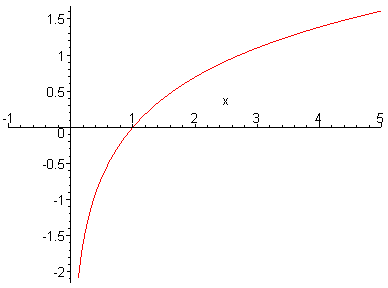
\includegraphics[scale=0.5]{./images/ln.png}
		\end{figure} 

		Область определения функции $(0, \infty)$. 
		\begin{enumerate}
			\item $\forall x \in (0, 1), f(x) \in (-\infty, 0)$
			\item $\text{Для } x = 1, f(x) := 0$
			\item $\text{Для } x = e, f(x) := 1$
			\item $\forall x \in (1, \infty), f(x) \in (0, \infty)$
			\item $\forall x \in (-\infty, 0), f(x) \in \varnothing$
		\end{enumerate}

    \subsection*{Модуль логарифмических функций}
		\subsubsection*{$lb$}
	    	\begin{figure}[h!]
    			\caption{График функции  двоичного логарифма}
    			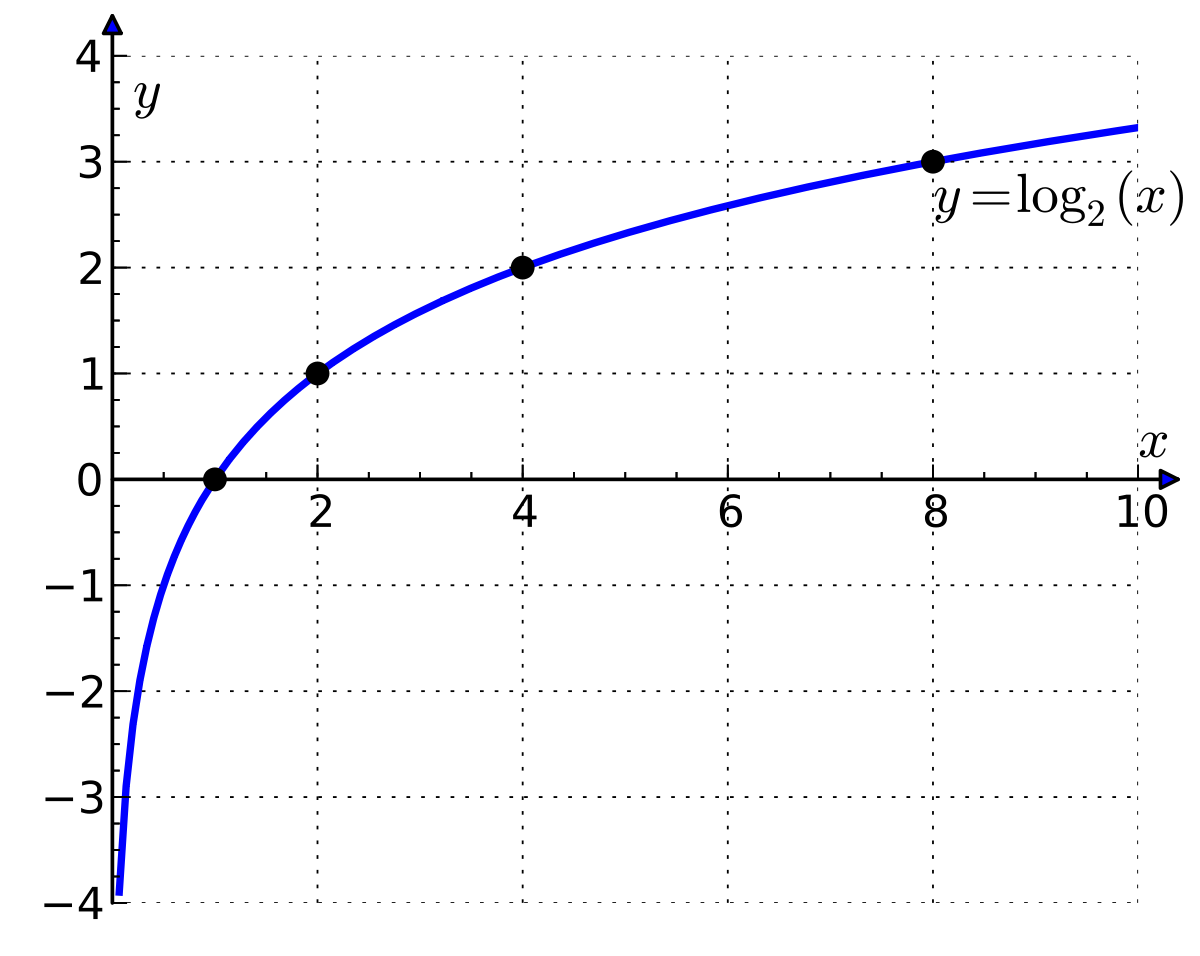
\includegraphics[scale=0.1]{./images/lb.png}
    		\end{figure} 
    		Функция выражена через натуральный логарифм: $lb(x) = ln(x)/ln(2)$.
    		Так как в данном модуле мы используем предположительно оттестированную функцию и математически обоснованное
    		преобразование функции, для тестирования функции двоичного логарифма достаточно оттестировать ряд значений,
    		являющихся степенью двойки.
		\subsubsection*{$log_3$}
	    	\begin{figure}[h!]
    			\caption{График функции  двоичного логарифма}
    			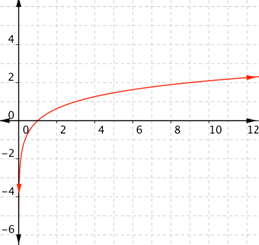
\includegraphics[scale=0.5]{./images/log3.png}
    		\end{figure} 
			Аналогично для логарифма по основанию 3.

    \subsection*{Модуль выражения с логарифмическими функциями}
		
		\begin{figure}[h!]
			\caption{График функции}
            \begin{tikzpicture}
                \begin{axis}[
                    domain=0.125:10,
                    xmin=0, xmax=7,
                    ymin=-200, ymax=200,
                    samples=500,
                    axis y line=center,
                    axis x line=middle,
                ]
                    \addplot+[mark=none] {ln(3)*(ln(x)^3)/(ln(2)^9)};
                \end{axis}
            \end{tikzpicture}
		\end{figure}

		Область определения функции $(0, \infty)$. 
		\begin{enumerate}
			\item $\forall x \in (0, 1), f(x) \in (-\infty, 0)$
			\item $\text{Для } x = 1, f(x) \in \varnothing$
			\item $\forall x \in (1, \infty), f(x) \in (0, \infty)$
			\item $\forall x \in (-\infty, 0), f(x) \in \varnothing$
		\end{enumerate}

    \subsection*{Модуль базовой функции $sin()$}
    \subsection*{Модуль тригонометрических функции} 
    \subsection*{Модуль выражения с тригонометрическими функциями}
    
\section*{Графики, полученные в процессе интеграции}
\section*{Вывод}

\end{document}
		\end{enumerate}
